% IEEE-formatted preliminary article (conference)
\documentclass[conference]{IEEEtran}
\usepackage[utf8]{inputenc}
\usepackage[T1]{fontenc}
\usepackage[english]{babel}
\usepackage{csquotes}
\usepackage{url}
\usepackage{graphicx}
\usepackage{microtype}
\usepackage{adjustbox}
\usepackage{rotating}
\usepackage{booktabs}
\usepackage{multirow}
\usepackage{cite}
\usepackage{hyperref}
\usepackage{amsmath}
\usepackage{tikz}
\renewcommand{\figurename}{Figura}
\usetikzlibrary{positioning, fit, arrows.meta, calc, patterns, decorations.pathreplacing}

\title{Tarea 1 - Señales, Sistemas y Procesamiento Digital de Señales}
\author{\IEEEauthorblockN{Zúñiga Ramírez Jose Eduardo}
\IEEEauthorblockA{Escuela de Ingeniería Electrónica \\
Instituto Tecnológico de Costa Rica \\
\{je.zuniga\}@estudiantec.cr}
}
\date{}

\begin{document}
\maketitle

% Loosen line breaking to avoid overfull boxes in two-column layout
\sloppy




%-----------------------------------------------
%     1. Muestreo y aliasing en señales musicales
%-----------------------------------------------

\section{Muestreo y aliasing en señales musicales}

\subsection{Pregunta a}
La frecuencia de muestreo es de 8kHz, el mismo enunciado lo indica al decir que el sistema captura audio a dicho valor.
La frecuencia de plegado o también llamado de Nyquist, se puede calcular por la ecuación \eqref{eq:nyquist}

\begin{equation}
F_{Nyquist} = \frac{F_s}{2}
\label{eq:nyquist}
\end{equation}


Sustituyendo $F_s = 8\,\text{kHz}$ en la ecuación \eqref{eq:nyquist}, se tiene que el valor de la frecuencia de plegado es de 4 kHz

\subsection{Pregunta b}

La nota musical más alta que puede grabar el sistema sin alias es de n = 38.
Este valor se obtuvo utilizando como referencia la ecuación \eqref{eq:nota}, que relaciona la frecuencia de una nota con el número de semitonos $n$ que la separan de La\textsubscript{4}.

\begin{equation}
F = 440 \cdot 2^{\frac{n}{12}}
\label{eq:nota}
\end{equation}

Esta ecuación se sustituye el valor de F por 4000 Hz y se resuelve con logaritmos para lograr despejar el valor de n. 
Al hacer el cálculo, n da un valor de 38.2 por lo que se debe obtar por un redondeo inferior para cumplir con la condición de frecuencia. 
Para encontrar la nota, se puede tomar de referencia la mayor nota que nos da el enunciado (Si\textsubscript{6} con n = 26) y contamos las posiciones hasta llegar a 38, siendo la mayor nota posible a capturar la Si\textsubscript{7}.


\subsection{Pregunta c}

Lo que sucederá en este caso es que se escuchará otra nota distinta a la esperada por el efecto de aliasing.
De acuerdo a la equivalencia enarmónica la nota del enunciado es equivalente al Re\#\textsubscript{8}, por lo que el valor de n es de 42. 

La frecuencia que se escuchará se obtiene de calcular primero la frecuencia correspondiente de la nota haciendo uso de la ecuación \eqref{eq:nota}, esto da un valor aproximado de 4978.03 Hz.
Luego se puede utilizar la ecuación normalizada de frecuencia que está dada por \eqref{eq:fnormalizada}, donde F = 4978.03 Hz y F\textsubscript{s} = 8000 Hz, obteniendo como resultado 0.6222.

\begin{equation}
f = \frac{F}{F_s}
\label{eq:fnormalizada}
\end{equation}

f debe de estar dentro del rango fundamental, por lo que para lograrlo se resta 1 al valor obtenido anteriormente. 
Se obtiene el valor de -0.3778 y se multiplica por F\textsubscript{s} para obtener el valor de frecuencia que se escuchará, siendo este de aproxiadamente 3022 Hz (siendo positivo debido a que no existen frecuencias negativas).
La nota más cercana a esta frecuencia es n = 33, que corresponde a Fa\textsubscript{7}

\subsection{Pregunta d}

El filtro anti-aliasing se encarga de eliminar las frecuencias superiores a la frecuencia de pliegue del sistema antes del muestreo.
Para esto se utiliza un filtro pasa bajas y soluciona el problema de que componentes de alta frecuencia se reflejen como notas falsas (para este ejemplo).
Como se evidencio en la pregunta c, si bien no pudimos capturar la nota de pícolo, se observa un equivalente o alias de la misma, dando un error en la señal.
%-----------------------------------------------
%     2. Visualización de una señal y su alias
%-----------------------------------------------

\section{Visualización de una señal y su alias}

Se implementó el script \texttt{Pregunta\_2.py}, que recibe como parámetros de usuario la frecuencia natural $F$, la frecuencia de muestreo $F_s$ y el número de ciclos a mostrar. 
El alias se calcula plegando $F$ al rango $[-F_s/2, F_s/2]$ mediante la operación módulo, y se grafica únicamente cuando difiere de $F$. 
Las muestras se obtienen evaluando la señal en $t=n/F_s$; al coincidir con la señal original y su alias en esos instantes, basta un único conjunto de puntos para representar ambas.

La Figura~\ref{fig:pregunta2} reproduce el ejemplo del enunciado ($F=5/7$ Hz, $F_s=1$ Hz, 7 ciclos), obteniendo $F_{\text{alias}}=-2/7$ Hz, igual al valor esperado.

\begin{figure}[h]
\centering
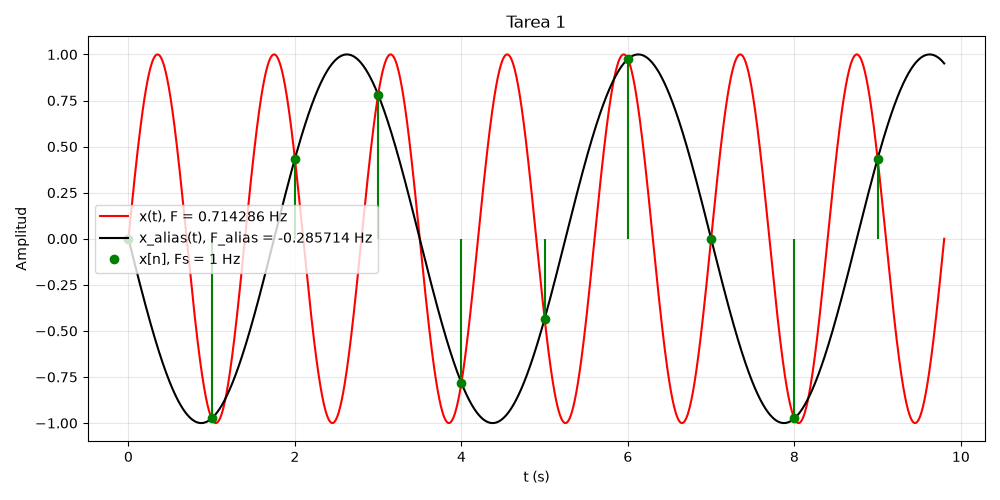
\includegraphics[width=\columnwidth]{figuras/pregunta2_resultado.png}
\caption{Señal $x(t)$, su alias $x_{\text{alias}}(t)$ y las muestras $x[n]$, para $F=5/7$ Hz, $F_s=1$ Hz.}
\label{fig:pregunta2}
\end{figure}

%-----------------------------------------------
%     3. Aliasing para recuperar la información de una señal modulada
%-----------------------------------------------

\section{Aliasing para recuperar la información de una señal modulada}

\subsection{Pregunta a}

Para expresar la señal de la ecuación \eqref{eq:xt} como una suma de tonos puros, se debe empezar por distribuir la multiplicación existente de la expresión.

\begin{equation}
x(t) = [1 + 0.5\cos(2\pi \cdot 100t)]\cos(2\pi \cdot 1000t),
\label{eq:xt}
\end{equation}

Al hacer la distribución se tiene el resultado de la ecuación \eqref{eq:xt_mult}

\begin{equation}
x(t) = cos(2\pi \cdot 1000t) + 0.5 cos(2\pi \cdot 100t)\cos(2\pi \cdot 1000t),
\label{eq:xt_mult}
\end{equation}

Tomando en cuenta la identidad trigonométrica de la ecuación \eqref{eq:identityTrig}, esta podemos aplicarla a la ecuación \eqref{eq:xt_mult} para llegar a la expresión de suma de tonos puros

\begin{equation}
cos(A)\cos(B)  = 0.5[cos(A+B)+cos(A-B)]
\label{eq:identityTrig}
\end{equation}

El resultado final está dado por la expresión de la ecuación \eqref{eq:xt_tonos}. 
En este se pueden identificar tres frecuencias: 900 Hz, 1000 Hz y 1100 Hz, la frecuencia de Nyquist debe tomar como la mayor frecuencia de estas para evitar el aliasing, siendo F\textsubscript{Nyquist} = 2200 Hz.

\begin{equation}
x(t) = \cos(2\pi \cdot 1000t) + 0.25\cos(2\pi \cdot 1100t) + 0.25\cos(2\pi \cdot 900t)
\label{eq:xt_tonos}
\end{equation}


\subsection{Pregunta b}

Para eliminar la oscilación de la portadora se debe muestrear a la misma frecuencia que esta, lo cual F\textsubscript{s} = 1000 Hz.
Esto es comparable al ejemplo de las aspas de un helicóptero, que cuando se está grabando y ambas frecuencias coinciden, pareciera que estas estuvieran detenidas. 
Matemáticamente se puede apreciar utilizando la ecuación \eqref{eq:fnormalizada}.


Para 1000 Hz que es la portadora se tiene que f = 1, debido a que F = F\textsubscript{s} = 1000 Hz, por lo tanto si restamos 1 a f para ajustar el valor dentro del rango fundamental, nos da como resultado 0.
Similarmente, para 1100 Hz se tiene que f = 1.1 y ajustandolo en el rango fundamental es 0.1, por lo tanto la frecuencia resultante es 100 Hz. 
Por ultimo para 900 Hz se tiene f = 0.9, haciendo el ajuste para el rango fundamental da -0.1 y la frecuencia vista es de -100 Hz.


\subsection{Pregunta c}

Para obtener x[n] se evaluan los nuevos valores de frecuencia en \eqref{eq:xt_tonos}, obteniendo \eqref{eq:xt_tonos_fn}

\begin{equation}
x(t) = \cos(2\pi \cdot 0t) + 0.25\cos(2\pi \cdot 100t) + 0.25\cos(2\pi \cdot (-100)t)
\label{eq:xt_tonos_fn}
\end{equation}

De la expresión anterior, para el primer termino al ser un argumento 0, el coseno toma el valor de 1. 
Para el segundo y tercer término, al ser el coseno una función par, el negativo de la frecuencia puede volverse positivo y ambas expresiones se pueden sumar por tener el mismo argumento. 
El resultado de esto se presenta en la ecuación \eqref{eq:xt_tonos_redux}, mientras que el mensaje m[n] está expresado en la ecuación \eqref{eq:msj}, en ambos casos se hace el cambio de variable $t=n/F_s$.

\begin{equation}
x[n] = 1 + 0.5\cos\left(2\pi \cdot 100 \cdot \frac{n}{F_s}\right)
\label{eq:xt_tonos_redux}
\end{equation}

\begin{equation}
m[n] = \cos\left(2\pi \cdot 100\cdot \frac{n}{F_s}\right)
\label{eq:msj}
\end{equation}


Con lo anterior podemos reescribir x(t) en terminos de m(t), obteniendo el resultado mostrado en la ecuación \eqref{eq:xt_tonos_wMsj}

\begin{equation}
x[n] = 1 + 0.5m[n]
\label{eq:xt_tonos_wMsj}
\end{equation}

Para recuperar m[n], se debe despejar la misma de la ecuación \eqref{eq:xt_tonos_wMsj}, este procedimiento es el siguiente:


$$m[n] = \frac{x[n]-1}{0.5} = 2\big(x[n]-1\big) = 2x[n]-2$$



\subsection{Pregunta d}

Para comprobar el resultado de forma numérica se implementó un script en Python (\texttt{Pregunta\_3.py}) que evalúa $x(t)$ directamente a partir de la ecuación \eqref{eq:xt} (sin utilizar la simplificación algebraica de las preguntas anteriores) en los instantes de muestreo $t=n/F_s$, con $F_s = 1000$ Hz. 
Sobre esas muestras $x[n]$ se aplicó el procedimiento de recuperación obtenido anteriormente, $m[n] = 2x[n]-2$, y el resultado se comparó contra $m[n]$ calculado directamente de $m(t) = \cos(2\pi \cdot 100t)$.

La Figura \ref{fig:pregunta3} muestra en la parte superior la señal $x(t)$ junto con sus muestras.
En la parte inferior el tono de información $m(t)$ junto con las muestras recuperadas mediante el procedimiento. 
Se representan tres ciclos del tono de 100 Hz (30 ms), con el eje horizontal expresado en milisegundos.

\begin{figure}[h]
\centering
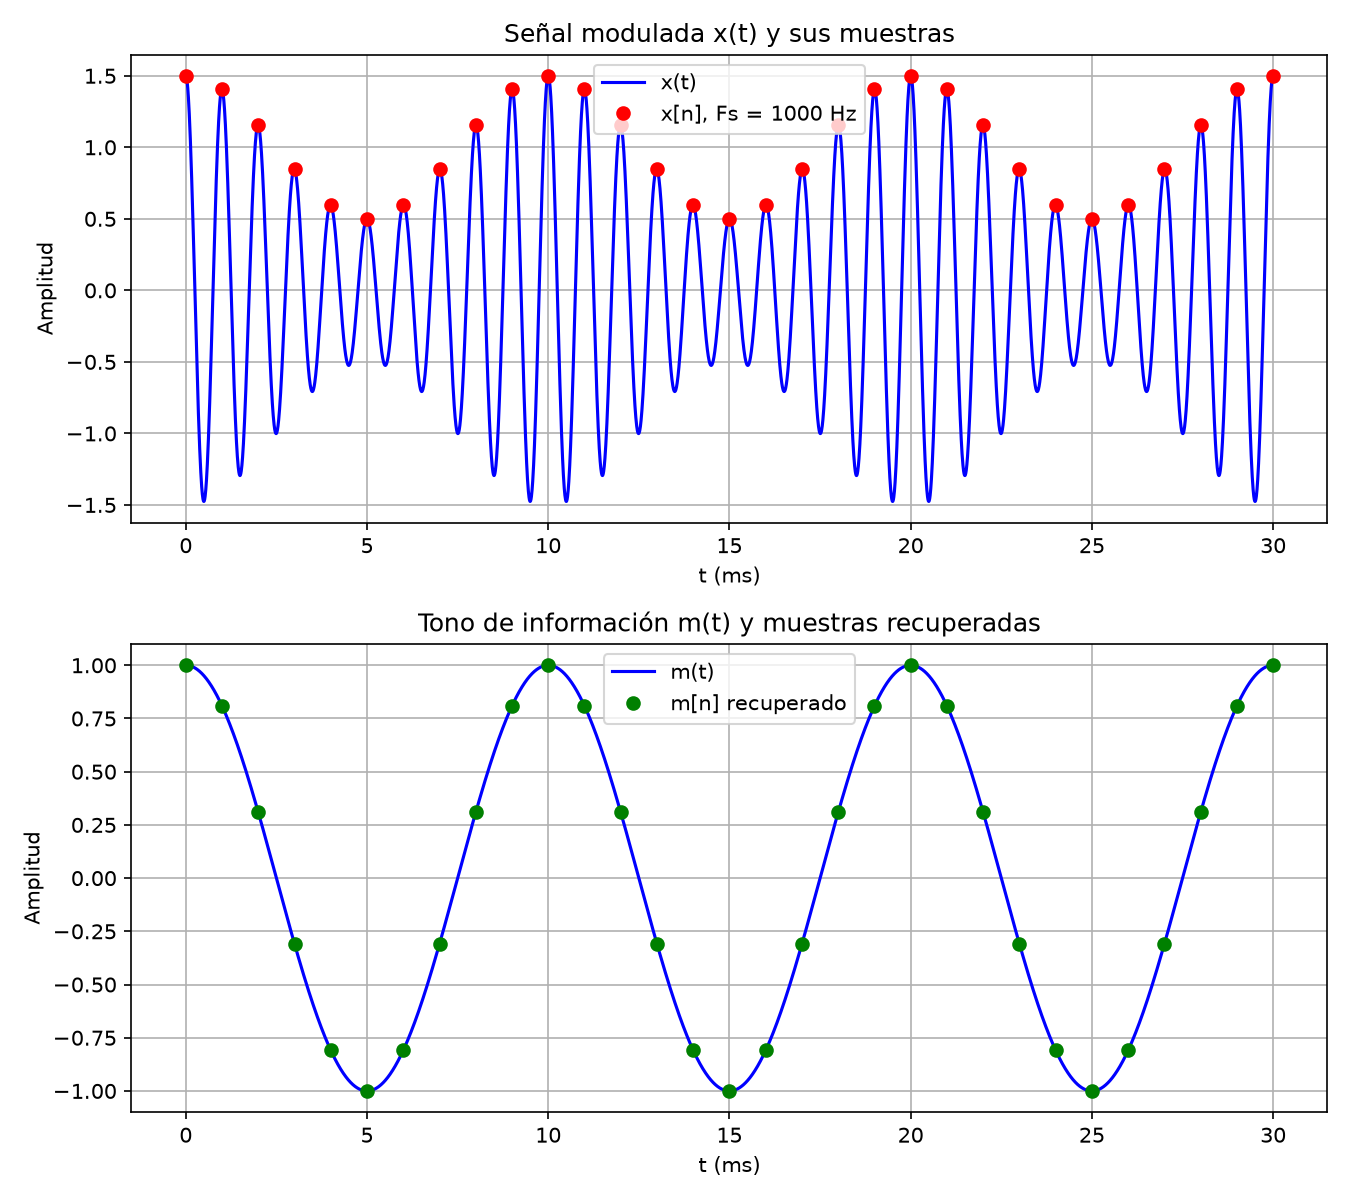
\includegraphics[width=\columnwidth]{figuras/pregunta3_resultado.png}
\caption{Señal $x(t)$ y sus muestras (arriba); tono de información $m(t)$ y las muestras recuperadas (abajo).}
\label{fig:pregunta3}
\end{figure}

Se obtuvieron 31 muestras con el método de recuperación y la misma cantidad de muestras calculadas apartir de la ecuación \eqref{eq:msj} y este retornó un error muy bajo debido a la naturaleza del punto flotante. 
si se recortan los resultados a 4 digitos después de la coma, se obtiene el mismo resultado en ambos casos, por lo que el método de recuperación es funcional.

\subsection{Pregunta e}

Para el caso en que se tiene una portadora con fase desconocida de forma como se muestra en la ecuación \eqref{eq:fase_desc}

\begin{equation}
x_\phi(t) = [1 + 0.5\cos(2\pi \cdot 100t)]\cos(2\pi \cdot 1000t + \phi)
\label{eq:fase_desc}
\end{equation}

Se puede distribuir la multiplicación y se puede aplicar la identidad trigonométrica de la ecuación \eqref{eq:identityTrig} tomando $A=2\pi\cdot100t$ y $B=2\pi\cdot1000t+\phi$. 
Además se puede utilizar la propiedad par del coseno para hacer la equivalencia $\cos(-2\pi\cdot900t-\phi)=\cos(2\pi\cdot900t+\phi)$, se obtiene:

\begin{equation}
\begin{aligned}
x_\phi(t) ={}& \cos(2\pi\cdot1000t+\phi) \\
              &+ 0.25\cos(2\pi\cdot900t+\phi) \\
              &+ 0.25\cos(2\pi\cdot1100t+\phi)
\end{aligned}
\label{eq:x_phi}
\end{equation}

La fase $\phi$ se traslada por igual a los tres tonos. 
Aplicando el plegado: $1000\,\text{Hz}\rightarrow0$, $900\,\text{Hz}\rightarrow-100$, $1100\,\text{Hz}\rightarrow+100$) y evaluando en $t=n/F_s$:


\begin{equation}
\begin{aligned}
x_\phi[n] ={}& \cos(\phi) \\
              &+ 0.25\cos\!\left(-2\pi\cdot100
              \frac{n}{F_s}+\phi\right) \\
              &+ 0.25\cos\!\left(2\pi\cdot100
              \frac{n}{F_s}+\phi\right)
\end{aligned}
\label{eq:x_phi_n}
\end{equation}

Usando $\cos(-\theta+\phi)=\cos(\theta-\phi)$ y la identidad suma-a-producto de cosenos $\cos(\theta-\phi)+\cos(\theta+\phi)=2\cos\theta\cos\phi$, la expresión se simplifica a:

\begin{equation}
x_\phi[n] = \cos(\phi)\big[1 + 0.5\,m[n]\big]
\label{eq:xphi_n}
\end{equation}

Aplicando el procedimiento de recuperación dado $m_{\text{calc}}[n]=2x_\phi[n]-2$, que asume $\phi=0$, sobre la ecuación \eqref{eq:xphi_n}:

\begin{equation}
m_{\text{calc}}[n] = 2\cos(\phi) + \cos(\phi)\,m[n] - 2
\label{eq:mcalc_phi}
\end{equation}

\textbf{Caso $\phi=\pi/3$:} con $\cos(\pi/3)=0.5$, la ecuación \eqref{eq:mcalc_phi} da $m_{\text{calc}}[n] = 0.5\,m[n]-1$. Se recupera una versión escalada a la mitad y desplazada de $m[n]$: la variación temporal de la información se conserva, pero el resultado no es $m[n]$ exacto a menos que se conozca $\phi$ para corregir la escala y el desplazamiento.

\textbf{Caso $\phi=\pi/2$:} con $\cos(\pi/2)=0$, la ecuación \eqref{eq:xphi_n} da $x_\phi[n]=0$ para todo $n$, y por lo tanto $m_{\text{calc}}[n]=-2$ (constante). La señal se anula por completo en los instantes de muestreo y se pierde toda la información, sin importar la forma de $m(t)$. Este es el caso de "nulo en cuadratura", donde la fase de muestreo queda desfasada 90° respecto a la portadora.

En conclusión, el procedimiento propuesto no permite recuperar la información para cualquier fase de la portadora. Solo funciona sin distorsión cuando $\phi=0$, para $\phi\neq0$ arbitrario el resultado queda escalado por $\cos(\phi)$ y desplazado, y en el caso $\phi=\pi/2$ la información se pierde totalmente.

%-----------------------------------------------
%     4. Cuantización y representación en punto fijo
%-----------------------------------------------

\section{Cuantización y representación en punto fijo}

\subsection{Pregunta a}

Con un procesador de 8 bits se dispone de $2^8=256$ niveles. 
El valor representado por nivel es de 23.53 mV, utilizando la aplicación de la ecuación \eqref{eq:quantum_a}:

\begin{equation}
\Delta_a = \frac{V_{max}-V_{min}}{L-1} = \frac{6\,\text{V}}{255} = 23.53\,\text{mV}
\label{eq:quantum_a}
\end{equation}

\subsection{Pregunta b}

En notación $Qm.n$ con complemento a dos, el rango representable es $[-2^{m-1},\,2^{m-1}-2^{-n}]$ y el cuanto es $2^{-n}$, con $m+n=8$. 
Para representar $[-3,3]\,\text{V}$ se necesita $2^{m-1}\geq3$.
Como $2^{m-1}$ es siempre una potencia de 2 y 3 no lo es, el menor valor posible es $2^{m-1}=4$, es decir $m=3$. Esto deja $n=8-3=5$ bits fraccionarios, dando el formato \textbf{Q3.5}:

\begin{equation}
\begin{aligned}
\Delta_b &= 2^{-5} = 0.03125\,\text{V} = 31.25\,\text{mV},\\
\text{rango} &= [-4,\ 3.96875]\,\text{V}
\end{aligned}
\label{eq:quantum_b}
\end{equation}

Comparando con la ecuación \eqref{eq:quantum_a}, el cuanto de la representación en punto fijo (31.25 mV) es mayor (de menor resolución) que el de la asignación directa del inciso a) (23.53 mV). 
Esto se debe a que el punto fijo en complemento a dos solo puede representar rangos cuyo límite es una potencia de 2 ($\pm4$ V en este caso), mientras que la señal del sensor únicamente necesita $\pm3$ V; el tramo entre 3 V y 4 V (y su simétrico) queda sin usarse, desperdiciando parte de los 256 códigos disponibles y reduciendo la resolución efectiva frente al inciso a), donde los 256 códigos se reparten exactamente sobre el rango útil.

\subsection{Pregunta c}

En punto fijo, tanto la suma como la multiplicación se realizan operando directamente sobre los códigos enteros almacenados (en complemento a dos), como si fueran números enteros normales.
La posición del punto binario se maneja de forma implícita, solo en la interpretación del resultado.
\begin{itemize}
    \item \textbf{Suma:} si dos números están en el mismo formato $Qm.n$ (mismo $n$), sus códigos enteros $A$ y $B$ se suman directamente y el resultado $A+B$ permanece en el mismo formato $Qm.n$, ya que la operación es lineal: $(A\cdot2^{-n})+(B\cdot2^{-n})=(A+B)\cdot2^{-n}$. 
    El problema es que la suma de dos números de $m$ bits puede necesitar $m+1$ bits para no perder información (crecimiento del rango dinámico), por lo que si el resultado se fuerza a los mismos $m$ bits originales puede producirse un \textit{overflow}.
    \item \textbf{Multiplicación:} al multiplicar dos números en formatos $Qm_1.n_1$ y $Qm_2.n_2$, los códigos enteros se multiplican directamente ($A\times B$), pero el resultado representa $(A\times B)\cdot2^{-(n_1+n_2)}$, es decir, queda en un formato $Q(m_1+m_2).(n_1+n_2)$: tanto la parte entera como la fraccionaria se duplican en ancho de bits. 
    El producto de dos números de 8 bits requiere hasta 16 bits para representarse sin pérdida.

\end{itemize}
\textbf{Dificultades al limitar el almacenamiento a 8 bits:} 
\begin{itemize}
    \item Desbordamiento, si el resultado excede el rango representable del formato de origen.
    \item Pérdida de precisión, al truncar o redondear los bits menos significativos del resultado extendido para que quepa de vuelta en 8 bits
    \item Necesidad de reajustar la posición del punto binario (desplazamiento de bits) cada vez que cambia el número de bits fraccionarios, con el riesgo de descartar bits significativos si no se hace con cuidado
\end{itemize}


\subsection{Pregunta d}

Cada medición del sensor está acotada al rango físico $[-3,3]\,\text{V}$.
\textbf{Suma:} la suma de dos mediciones puede tomar valores en $[-6,6]\,\text{V}$. Se requiere $2^{m-1}\geq6$, y la menor potencia de 2 que cumple es $2^{m-1}=8$, es decir $m=4$. Con 8 bits totales, $n=8-4=4$, dando el formato \textbf{Q4.4}:

\begin{equation}
\begin{aligned}
\Delta_{suma} &= 2^{-4} = 0.0625\,\text{V} = 62.5\,\text{mV},\\
\text{rango} &= [-8,\ 7.9375]\,\text{V}
\end{aligned}
\label{eq:quantum_suma}
\end{equation}

\textbf{Multiplicación:} el producto de dos mediciones puede tomar valores en $[-9,9]\,\text{V}^2$ (el máximo se alcanza en $(\pm3)\times(\mp3)$ o $(\pm3)\times(\pm3)$). Se requiere $2^{m-1}\geq9$, y la menor potencia de 2 que cumple es $2^{m-1}=16$, es decir $m=5$. Con 8 bits totales, $n=8-5=3$, dando el formato \textbf{Q5.3}:

\begin{equation}
\begin{aligned}
\Delta_{producto} &= 2^{-3} = 0.125\,\text{V} = 125\,\text{mV},\\
\text{rango} &= [-16,\ 15.875]\,\text{V}
\end{aligned}
\label{eq:quantum_producto}
\end{equation}

En ambos casos se eligió el menor $m$ posible que cubre el rango físico de la operación, maximizando así los bits fraccionarios $n$ disponibles (y por lo tanto la resolución) dentro del presupuesto fijo de 8 bits. Nótese que, al tener que ceder bits enteros para cubrir el crecimiento del rango dinámico, ambos formatos resultan con menor resolución que el formato Q3.5 del inciso b) usado para las mediciones individuales.

\subsection{Pregunta e}

Para una señal senoidal de amplitud $A=3\,\text{V}$, la potencia de la señal es $A^2/2=4.5\,\text{W}$. Considerando cuantización por redondeo con error uniforme de varianza $\Delta^2/12$, la relación señal a ruido de cuantización es:

\begin{equation}
\begin{aligned}
\text{SQNR (dB)}
&= 10\log_{10}\!\left(
\frac{A^2/2}{\Delta^2/12}
\right) \\
&= 10\log_{10}(6)
+ 20\log_{10}\!\left(\frac{A}{\Delta}\right)
\end{aligned}
\label{eq:sqnr}
\end{equation}

Sustituyendo el cuanto $\Delta$ de cada formato obtenido en los incisos anteriores en la ecuación \eqref{eq:sqnr}:

\begin{itemize}
\item Inciso a) ($\Delta_a = 6/255\,\text{V}$): SQNR $\approx 49.89$ dB
\item Inciso b) ($\Delta_b = 0.03125\,\text{V}$, formato Q3.5): SQNR $\approx 47.43$ dB
\item Inciso d), suma ($\Delta_{suma} = 0.0625\,\text{V}$, formato Q4.4): SQNR $\approx 41.41$ dB
\item Inciso d), producto ($\Delta_{producto} = 0.125\,\text{V}$, formato Q5.3): SQNR $\approx 35.39$ dB
\end{itemize}

La pérdida de aproximadamente 6 dB entre formatos consecutivos corresponde exactamente a la pérdida de 1 bit de resolución fraccionaria ($6.02\,\text{dB/bit}$, consistente con la regla práctica $\text{SQNR}\approx6.02B+1.76$ dB): de b) a suma se pierde 1 bit fraccionario (6.02 dB) y de b) a producto se pierden 2 bits (12.04 dB), confirmando que representar la misma señal de 3 V en un formato pensado para un rango dinámico mayor (como los de suma o producto) sacrifica resolución y, por lo tanto, calidad de cuantización.


%-----------------------------------------------
%     5. Investigación de un caso de conducción temeraria
%-----------------------------------------------

\section{Investigación de un caso de conducción temeraria}

\subsection{Antecedentes}

La tarjeta de memoria dañada de la cámara solo permitió recuperar 1 de cada 15 cuadros del video original, y a partir de ellos los investigadores estimaron una velocidad aparente de 47 km/h siguiendo el desplazamiento de la línea blanca discontinua entre cuadros. 
Sin embargo, esta demarcación no es una marca continua sino un patrón espacial periódico, y perder 14 de cada 15 cuadros equivale a submuestrear dicho patrón aplicado ahora al dominio espacial en vez del temporal. 
Esto plantea la posibilidad de que la lectura de 47 km/h sea, en realidad, un alias de una velocidad mayor. 
Este informe evalúa dicha hipótesis y la contrasta con la evidencia de localización celular.

\subsection{Fuentes consultadas}

\begin{itemize}
\item Especificación del fabricante: Garmin Dash Cam Mini 2, grabación 1080p hasta 30 fps \cite{garmin2024}.
\item Manual Centroamericano de Dispositivos Uniformes para el Control del Tránsito (SIECA/MOPT), Sección 3.2.2 (líneas de carril): para carreteras rurales, segmentos de 4.5 m y espacios de 7.5 m \cite{sieca2014}.
\item Identificación de la autopista Florencio del Castillo como tramo interurbano de la Ruta 2, y no una calle urbana \cite{ruta2wiki}.
\item Descripción del fenómeno de aliasing espacial en patrones periódicos (\textit{wagon-wheel effect}), como referencia conceptual del efecto que se explota en este análisis \cite{wagonwheel}.
\end{itemize}

\subsection{Supuestos}

\begin{itemize}
\item La cámara capturó a su tasa nominal de 30 fps antes de la pérdida de cuadros.
\item El periodo de la demarcación es $D=12$ m, según la clasificación de carretera rural de la fuente SIECA/MOPT. 
Este es el supuesto de mayor incertidumbre del informe, al no haberse confirmado el valor exacto para este tramo específico.
\item El vehículo se desplazó por la vía que conecta ambos puntos de localización celular.
\item La posición real del teléfono en cada medición está dentro del radio de incertidumbre reportado.
\end{itemize}

\subsection{Metodología}

\subsubsection{Aliasing espacial en el video}

Con la tasa nominal de 30 fps y una recuperación de 1 de cada 15 cuadros, la tasa efectiva de la evidencia es $f_{\text{eff}}=30/15=2$ fps, es decir $T_{\text{eff}}=0.5$ s entre cuadros recuperados. 
Como la demarcación es un patrón espacial periódico de periodo $D=12$ m, un desplazamiento real de un múltiplo entero de $D$ dentro de $T_{\text{eff}}$ resulta indistinguible de no haberse movido. 
Esto implica que la velocidad aparente de 47 km/h admite como velocidades reales candidatas:

\begin{equation}
v_k = 47 + \frac{D}{T_{\text{eff}}}\cdot 3.6\,k = 47 + 86.4\,k \ \text{km/h}, \quad k=0,1,2,\dots
\label{eq:alias_velocidad}
\end{equation}

es decir $v_0=47$, $v_1=133.4$, $v_2=219.8$ y $v_3=306.2$ km/h.

\subsubsection{Localización celular como desambiguador}

Usando las coordenadas de ambas torres y la fórmula de Haversine, la distancia en línea recta entre los dos puntos es de 2499.4 m, lo que en los 60 s transcurridos da una velocidad promedio central de $2499.4\,\text{m}/60\,\text{s}\times3.6\approx150.0$ km/h. 
Tomando el caso más conservador sumando ambos radios de incertidumbre ($600+900=1500$ m) como holgura sobre esa distancia, el rango de velocidad compatible con esta evidencia es $[60,\ 240]$ km/h.

\subsection{Resultados}

Comparando ambas piezas de evidencia, $v_0=47$ km/h queda fuera del rango celular y se descarta, al igual que $v_3=306.2$ km/h. 
De las dos candidatas restantes, $v_1=133.4$ km/h y $v_2=219.8$ km/h, la primera es considerablemente más cercana a la estimación central de 150.0 km/h (16.6 km/h de diferencia, frente a 69.8 km/h de la segunda), por lo que se selecciona como la velocidad real del vehículo.

\subsection{Incertidumbre y limitaciones}

El valor asumido $D=12$ m para el periodo de la demarcación es la mayor fuente de incertidumbre: cada metro de diferencia desplazaría la candidata seleccionada en $\pm7.2$ km/h, por lo que idealmente debería confirmarse contra el estándar oficial de COSEVI/MOPT para este tramo específico. 
Además, la distancia obtenida de las torres celulares se aproximó como una línea recta entre los dos puntos; si la vía real tiene curvas, la distancia recorrida (y por tanto la velocidad) sería aún mayor, lo cual reforzaría esta conclusión en vez de contradecirla.

\subsection{Conclusión}

La lectura de 47 km/h es un artefacto de aliasing espacial producido por la pérdida de cuadros del video. 
La evidencia de localización celular permite descartar esa lectura literal y seleccionar el primer alias físicamente consistente. 
La velocidad estimada del sospechoso es:

\begin{equation}
v \approx 133\ \text{km/h} \pm 10\ \text{km/h}
\label{eq:velocidad_final}
\end{equation}

\bibliographystyle{IEEEtran}
\bibliography{references}

\end{document}

